% Set up the standalone document clas
\documentclass{standalone}

% Input the preamble (<3)
% Preamble document

% Import tikz package
\usepackage{tikz}

% Import tikz libraries
\usetikzlibrary{shapes, arrows}
\usetikzlibrary{positioning, calc}

%----------- Create a fancy summing block
\tikzset{add/.style n args={4}{
		minimum width=6mm,
		path picture={
			\draw[black] 
			(path picture bounding box.south east) -- (path picture bounding box.north west)
			(path picture bounding box.south west) -- (path picture bounding box.north east);
			\node at ($(path picture bounding box.south)+(0,0.13)$)     {\tiny #1};
			\node at ($(path picture bounding box.west)+(0.13,0)$)      {\tiny #2};
			\node at ($(path picture bounding box.north)+(0,-0.13)$)    {\tiny #3};
			\node at ($(path picture bounding box.east)+(-0.13,0)$)     {\tiny #4};
		}
	}
}

%----------- Block style 1
\tikzstyle{block1} = [draw, fill=blue!20, rectangle, 
minimum height=3em, minimum width=6em, node distance=2.5cm]

%----------- Block style 2
\tikzstyle{block2} = [draw, fill=blue!20, rectangle, 
minimum height=3em, minimum width=3em, node distance=2.5cm]

%----------- Sum style
\tikzstyle{sum} = [draw, fill=blue!20, circle, node distance=2cm]

%----------- Input style
\tikzstyle{input} = [coordinate, node distance=4cm]

%----------- Output style
\tikzstyle{output} = [coordinate, node distance=4cm]

%----------- Pin style
\tikzstyle{pinstyle} = [pin edge={to-,thin,black}]

\usepackage{amsmath}

% Additional styles
\tikzstyle{blockn} = [rectangle, draw, text width=8em, text centered, rounded corners, minimum height=4em]
    
\tikzstyle{line} = [draw, -latex]

\tikzset{
    block/.style={
        draw,
        rectangle split,
        rectangle split parts=2,
        text centered,
        text width=8em,
        rounded corners,
        minimum height=4em
        }
}

\begin{document}
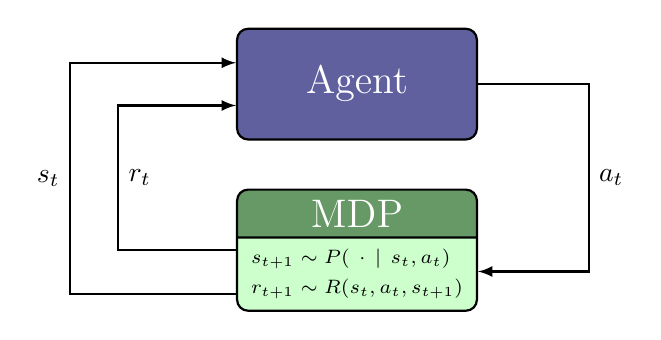
\begin{tikzpicture}[node distance = 6em, auto, thick]
    \node [blockn, fill=blue!25!gray, text=white] (Agent) {\Large Agent};
    \node [block, below of=Agent, rectangle split empty part height=1cm, rectangle split part fill={green!20!gray,white!80!green}] (Environment) {\Large\textcolor{white}{MDP} \nodepart{second} \scriptsize $\begin{aligned}
   		s_{t+1} &\sim  P( \ \cdot \ | \ s_t,a_t )\\
   		r_{t+1} &\sim R(s_t, a_t, s_{t+1})
    \end{aligned}$};
    
    \path [line] (Agent.0) --++ (4em,0em) |- node [near start]{$a_t$} (Environment.-10);
    \path [line] (Environment.200) --++ (-6em,0em) |- node [near start] {$s_t$} (Agent.170);
    \path [line] (Environment.180) --++ (-4.25em,0em) |- node [near start, right] {$r_t$} (Agent.190);
\end{tikzpicture}
\end{document}